\documentclass[11pt]{amsart}
\usepackage{amsmath}
\usepackage{amssymb}
\usepackage{tikz}
\usetikzlibrary{patterns}

\begin{document}

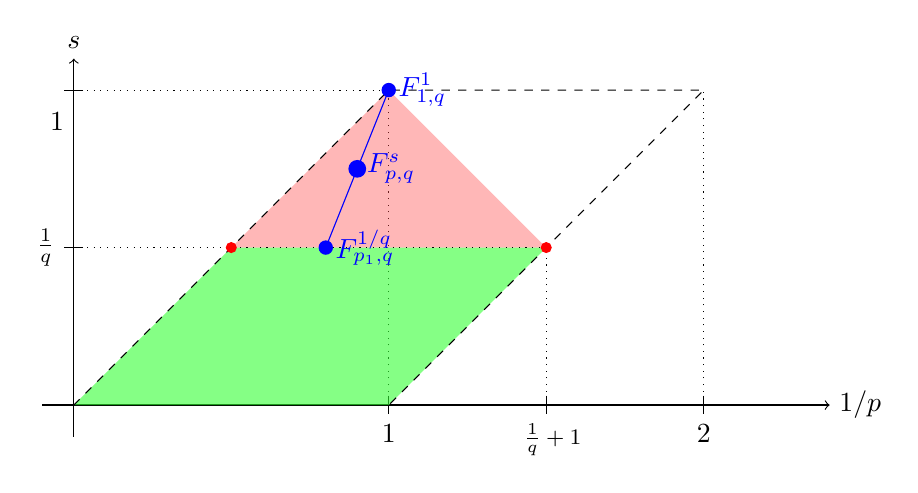
\begin{tikzpicture}[scale=4]


% Axes
\draw[->] (-0.1,0.0) -- (2.4,0.0) node[right] {${1}/{p}$};
\draw[->] (0.0,-0.1) -- (0.0,1.1) node[above] {$s$};


% Ticks
\draw (1.0,0.03) -- (1.0,-0.03) node [below] {$1$};
\draw (2.0,0.03) -- (2.0,-0.03) node [below] {$2$};
\draw (1.5,0.03) -- (1.5,-0.03) node [below] {{\footnotesize $\;\;\frac1q+1$}};
\draw (0.03,1.0) -- (-0.03,1.00);
\node [left] at (0,0.9) {$1$};
\draw (0.03,.5) -- (-0.03,.5) node [left] {$\tfrac{1}{q}$};



% Plot
\draw[dotted] (1.0,0.0) -- (1.0,1.0);
\draw[dotted] (0,1.0) -- (1.0,1.0);
\draw[dotted] (1.5,0.0) -- (1.5,0.5);
\draw[dotted] (2,0.0) -- (2,1.0);

\path[fill=red!70, opacity=0.4] 
(.5,.5)-- (1.5,0.5) -- (1,1);


\path[fill=green!80, dashed, opacity=0.6] (0.0,0.0) -- (.5,.5)-- (1.5,0.5) -- (1,0)--(0,0);
\draw[dotted] (0,0.5)--(1.5,0.5);

\draw[dashed] (0.0,0.0) -- (1.0,1.0) -- (2,1.0) -- (1.0,0.0);

\fill[blue] (1,1) circle (0.65pt) node [right] {$F^1_{1,q}$};
\fill[red] (0.5,0.5) circle (0.5pt);
\fill[red] (1.5,0.5) circle (0.5pt);

\fill[blue] (0.8,0.5) circle (0.65pt) node [right] {$F^{1/q}_{p_1,q}$};
\draw[blue] (0.8,0.5)--(1,1);
\fill[blue] (0.9,0.75) circle (0.8pt) node [right] {$F^s_{p,q}$};

\end{tikzpicture}

\end{document}